%Adapted from source: https://tex.stackexchange.com/a/525820
\documentclass[tikz, border = 3mm]{standalone}
\usetikzlibrary{chains, shapes.symbols}

\begin{document}
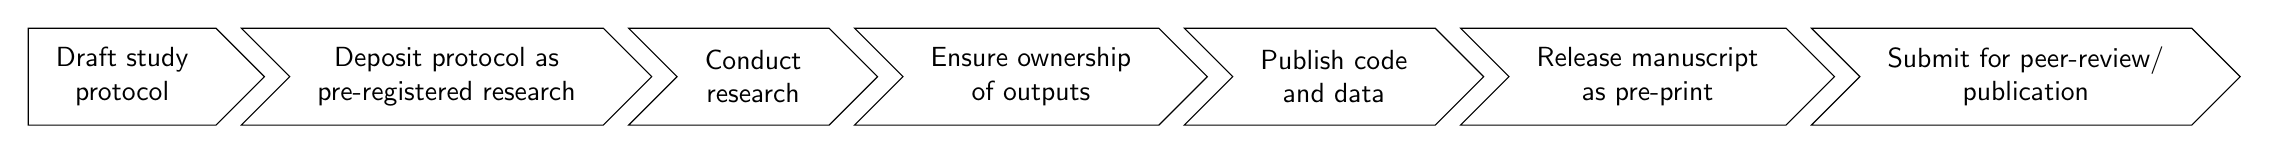
\begin{tikzpicture}[nodes = {shape = signal,signal from = west, signal to = east,
    align = center, draw = black, font = \sffamily, on chain, minimum height = 3.5em,
    inner xsep = 1em}, start chain = going right, node distance = 2ex]
 \path node[signal from = nowhere]{Draft study\\ protocol}
 
 node{Deposit protocol as\\ pre-registered research}
 
 node{Conduct\\ research}
 
 node{Ensure ownership\\ of outputs}
 
 node{Publish code\\ and data}
 
 node{Release manuscript\\ as pre-print}
 
 node{Submit for peer-review/\\publication};
 \end{tikzpicture}

\end{document}
